\section{Results}
The results are divided into two groups, simple simulation and advanced simulation.
\subsection{Results with simple simulation}
The simple simulation is characterized by sensors being spread evenly throughout the map. The rule is that a sensor cannot touch another sensor. The figure below illustrates the success of the fire interpreter. The light green color is where the actual fire is and where the interpreter predicted it to be. Therefore the color of success. The dark green color is area where the interpreter thought it would be fire, but was not. The red parts are the actual fire which the interpreter did not predict. When using the simple simulator each sensor can only sense its closest neighbours. 
\begin{figure}[here]
  \centering
      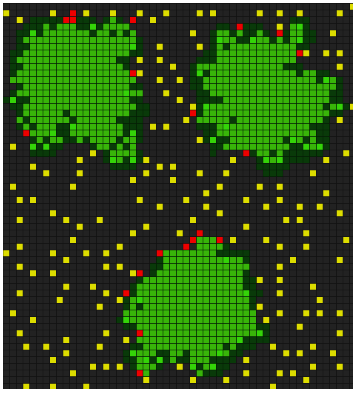
\includegraphics[width=0.5\textwidth]{discussion/graphics/results-simple-compare.png}
  \caption{The intense green is where the fire interpreter predicted correctly. The dark green is where the fire interpreter thought it was fire, but it was not. Red dots are where there actually was fire, but the predictor was unable to predict it.}
  \label{fig:simple-results1}
\end{figure}


\subsection{Results with advanced simulation}
The advanced simulation mimics the effect of humidity and wind has on a fire. The sensors are spread more randomly than in the simple simulation. They can also sense with a larger range. The default is two cells. In these tests wind were enabled in the interpreter to better cope with the wind in the simulation. The illustration below has the real fire on the left together with the sensor (yellow dot) and on the right interpreter prediction.

\begin{figure}[here]
  \centering
      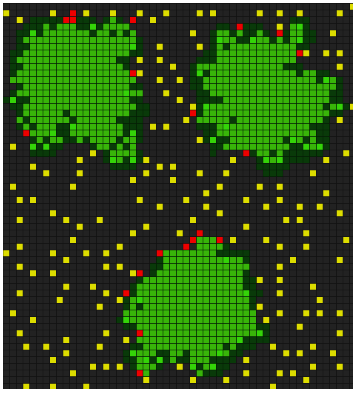
\includegraphics[width=0.5\textwidth]{discussion/graphics/results-simple-compare.png}
  \caption{The intense green is where the fire interpreter predicted correctly. The dark green is where the fire interpreter thought it was fire, but it was not. Red dots are where there actually was fire, but the predictor was unable to predict it.}
  \label{fig:advanced-results1}
\end{figure}